% This LaTeX was auto-generated from MATLAB code.
% To make changes, update the MATLAB code and export to LaTeX again.

\documentclass{article}

\usepackage[utf8]{inputenc}
\usepackage[T1]{fontenc}
\usepackage{lmodern}
\usepackage{graphicx}
\usepackage{color}
\usepackage{hyperref}
\usepackage{amsmath}
\usepackage{amsfonts}
\usepackage{epstopdf}
\usepackage[table]{xcolor}
\usepackage{matlab}
\usepackage[paperheight=795pt,paperwidth=614pt,top=72pt,bottom=72pt,right=72pt,left=72pt,heightrounded]{geometry}

\sloppy
\epstopdfsetup{outdir=./}
\graphicspath{ {./E23_media/} }

\begin{document}

\matlabtitle{62743 DSP — E23 Exam}

\begin{matlabcode}
%% 62743 DSP — E23 Exam
%  MATLAB Live Script companion
%
%  This script generates all figures referenced in:
%  "62743 — E23 Exam (Digital Signal Processing).md"
%
%  Images are exported to your Obsidian DSP image folder.
%
%  UPDATE: Added positivity verification for Q1-3 (linear phase justification)

clear; close all; clc;

%% Global image directory (Obsidian path)

imgDir = 'C:\Users\Mads2\DTU\Obsidian\Courses\DSP\Images';
if ~exist(imgDir, 'dir')
    mkdir(imgDir);
end

delta = @(k) double(k == 0);
u     = @(k) double(k >= 0);


\end{matlabcode}


\matlabheading{Problem 1 — LTI step → impulse, symmetry \& cascade}

\begin{matlabcode}


%% 1-1) Impulse response from step response
% Time indices (a little larger than strictly needed)
n = 0:10;

% Given step-response output y1[n] for input x1[n] = u[n]
% (from E23 solution sheet)
%   y1[n] = -δ[n] - 5δ[n-1] + 5δ[n-2] + δ[n-3]
y1 = -delta(n) - 5*delta(n-1) + 5*delta(n-2) + delta(n-3);

% For an LTI system: δ[n] = u[n] - u[n-1] ⇒ h[n] = y1[n] - y1[n-1]
y1_shift = [0, y1(1:end-1)];
h = y1 - y1_shift;

fprintf('1-1) Impulse response h[n] from step response:\n');
\end{matlabcode}
\begin{matlaboutput}
1-1) Impulse response h[n] from step response:
\end{matlaboutput}
\begin{matlabcode}
disp(table(n.', h.', 'VariableNames', {'n','h'}));
\end{matlabcode}
\begin{matlaboutput}
    n     h 
    __    __

     0    -1
     1    -4
     2    10
     3    -4
     4    -1
     5     0
     6     0
     7     0
     8     0
     9     0
    10     0
\end{matlaboutput}
\begin{matlabcode}

figure;
stem(n, h, 'filled'); grid on;
xlabel('n'); ylabel('h[n]');
title('E23: Problem 1-1 — Impulse response h[n]');
exportgraphics(gcf, fullfile(imgDir, ...
    'DSP_Exam_E23_1_ImpulseResponse.png'), 'Resolution', 300);
\end{matlabcode}
\begin{center}
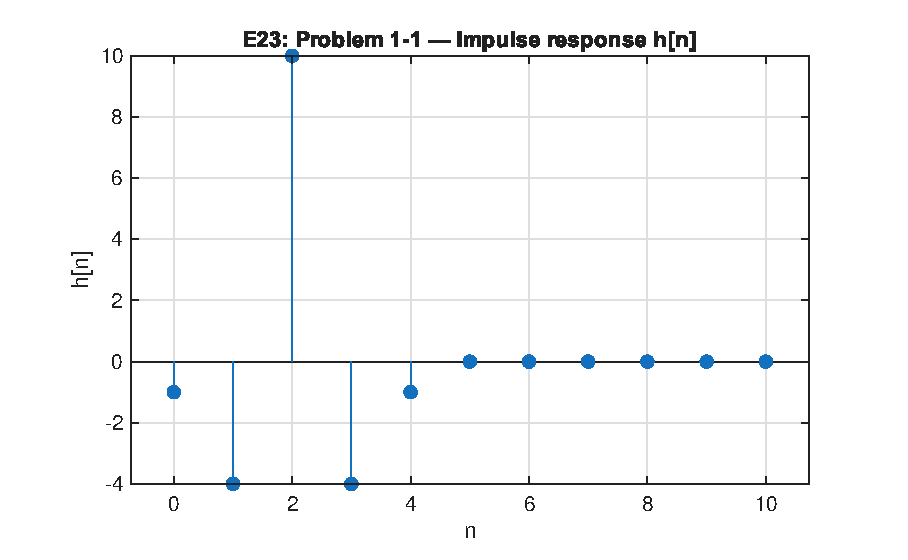
\includegraphics[width=\maxwidth{56.196688409433015em}]{figure_0.eps}
\end{center}
\begin{matlabcode}


\end{matlabcode}


\matlabheading{1-2) System function H(z) and frequency response H(ω)}

\begin{matlabcode}

% Keep only the non-zero support (0..4)
h = h(1:5);                % h[0..4] = [-1 -4 10 -4 -1]
B = h;                     % FIR numerator
A = 1;                     % denominator

fprintf('\n1-2) H(z) numerator coefficients (overall FIR):\n');
\end{matlabcode}
\begin{matlaboutput}
1-2) H(z) numerator coefficients (overall FIR):
\end{matlaboutput}
\begin{matlabcode}
disp(B);
\end{matlabcode}
\begin{matlaboutput}
    -1    -4    10    -4    -1
\end{matlaboutput}
\begin{matlabcode}

Nw = 2048;
[H_omega, w_full] = freqz(B, A, Nw, 'whole');   % 0..2π


\end{matlabcode}


\matlabheading{1-3) Magnitude / phase from symmetry vs freqz — WITH POSITIVITY CHECK}

\begin{matlabcode}

W = linspace(-pi, pi, 4001);

% Analytic magnitude for symmetric length-5 FIR:
% H(ω) = e^{-j2ω} (10 - 8 cos ω - 2 cos 2ω)
% Define the AMPLITUDE FUNCTION A(ω)
A_omega = 10 - 8*cos(W) - 2*cos(2*W);
phase_analytic = -2*W;      % linear phase (ONLY valid if A(ω) >= 0!)

% =========================================================================
%  CRITICAL UPDATE: Positivity Verification for Linear Phase Claim
%  Must verify A(ω) >= 0 for all ω ∈ [-π, π] before claiming phase = -2ω
% =========================================================================
fprintf('\n1-3) POSITIVITY CHECK for A(ω) — Required for linear phase claim:\n');
\end{matlabcode}
\begin{matlaboutput}
1-3) POSITIVITY CHECK for A(ω) — Required for linear phase claim:
\end{matlaboutput}
\begin{matlabcode}
fprintf('=====================================================================\n');
\end{matlabcode}
\begin{matlaboutput}
=====================================================================
\end{matlaboutput}
\begin{matlabcode}
fprintf('  A(0)      = %6.2f   (should be >= 0)\n', 10 - 8*cos(0) - 2*cos(0));
\end{matlabcode}
\begin{matlaboutput}
  A(0)      =   0.00   (should be >= 0)
\end{matlaboutput}
\begin{matlabcode}
fprintf('  A(π/2)    = %6.2f   (should be >= 0)\n', 10 - 8*cos(pi/2) - 2*cos(pi));
\end{matlabcode}
\begin{matlaboutput}
  A(π/2)    =  12.00   (should be >= 0)
\end{matlaboutput}
\begin{matlabcode}
fprintf('  A(π)      = %6.2f   (should be >= 0)\n', 10 - 8*cos(pi) - 2*cos(2*pi));
\end{matlabcode}
\begin{matlaboutput}
  A(π)      =  16.00   (should be >= 0)
\end{matlaboutput}
\begin{matlabcode}
fprintf('  min(A(ω)) = %6.4f   (MUST be >= 0 for no phase jumps)\n', min(A_omega));
\end{matlabcode}
\begin{matlaboutput}
  min(A(ω)) = 0.0000   (MUST be >= 0 for no phase jumps)
\end{matlaboutput}
\begin{matlabcode}
fprintf('=====================================================================\n');
\end{matlabcode}
\begin{matlaboutput}
=====================================================================
\end{matlaboutput}
\begin{matlabcode}

if min(A_omega) >= -1e-10  % small tolerance for numerical errors
    fprintf('  ✓ VERIFIED: A(ω) >= 0 for all ω ∈ [-π, π]\n');
    fprintf('  ✓ Therefore: ∠H(ω) = -2ω (pure linear phase, no jumps)\n');
else
    fprintf('  ✗ WARNING: A(ω) goes negative! Phase will have ±π jumps!\n');
end
\end{matlabcode}
\begin{matlaboutput}
  ✓ VERIFIED: A(ω) >= 0 for all ω ∈ [-π, π]
  ✓ Therefore: ∠H(ω) = -2ω (pure linear phase, no jumps)
\end{matlaboutput}
\begin{matlabcode}
fprintf('\n');

% Shift freqz result to [-π, π]
w_shift = w_full - pi;
H_shift = fftshift(H_omega);

% Create figure with 3 subplots (added zoomed positivity check)
figure('Position', [100 100 800 700]);

subplot(3,1,1);
plot(W, A_omega, 'LineWidth', 1.5); hold on;
plot(w_shift, abs(H_shift), '--', 'LineWidth', 1.0);
yline(0, '--r', 'LineWidth', 1.0);
scatter(0, 0, 80, 'ro', 'filled');  % Mark where A touches zero
grid on;
xlabel('\omega [rad/sample]');
ylabel('|H(\omega)| = A(\omega)');
legend('Analytic A(\omega)','freqz |H|','Zero line','A(0)=0','Location','best');
title('E23: Problem 1-3 — Magnitude (VERIFY A(\omega) \geq 0)');

subplot(3,1,2);
plot(W, phase_analytic, 'LineWidth', 1.5); hold on;
plot(w_shift, unwrap(angle(H_shift)), '--', 'LineWidth', 1.0);
grid on;
xlabel('\omega [rad/sample]');
ylabel('\angle H(\omega) [rad]');
legend('Analytic -2\omega','freqz','Location','best');
title('E23: Problem 1-3 — Phase response (linear, no jumps since A(\omega) \geq 0)');

subplot(3,1,3);
W_zoom = linspace(-0.5, 0.5, 501);
A_zoom = 10 - 8*cos(W_zoom) - 2*cos(2*W_zoom);
plot(W_zoom, A_zoom, 'b-', 'LineWidth', 1.5); hold on;
yline(0, '--r', 'LineWidth', 1.0);
scatter(0, 0, 100, 'ro', 'filled');
grid on;
xlabel('\omega [rad/sample]');
ylabel('A(\omega)');
title('Zoomed: A(\omega) touches zero at \omega=0 but never goes negative');
xlim([-0.5, 0.5]);

exportgraphics(gcf, fullfile(imgDir, ...
    'DSP_Exam_E23_1_MagPhase.png'), 'Resolution', 300);
\end{matlabcode}
\begin{center}
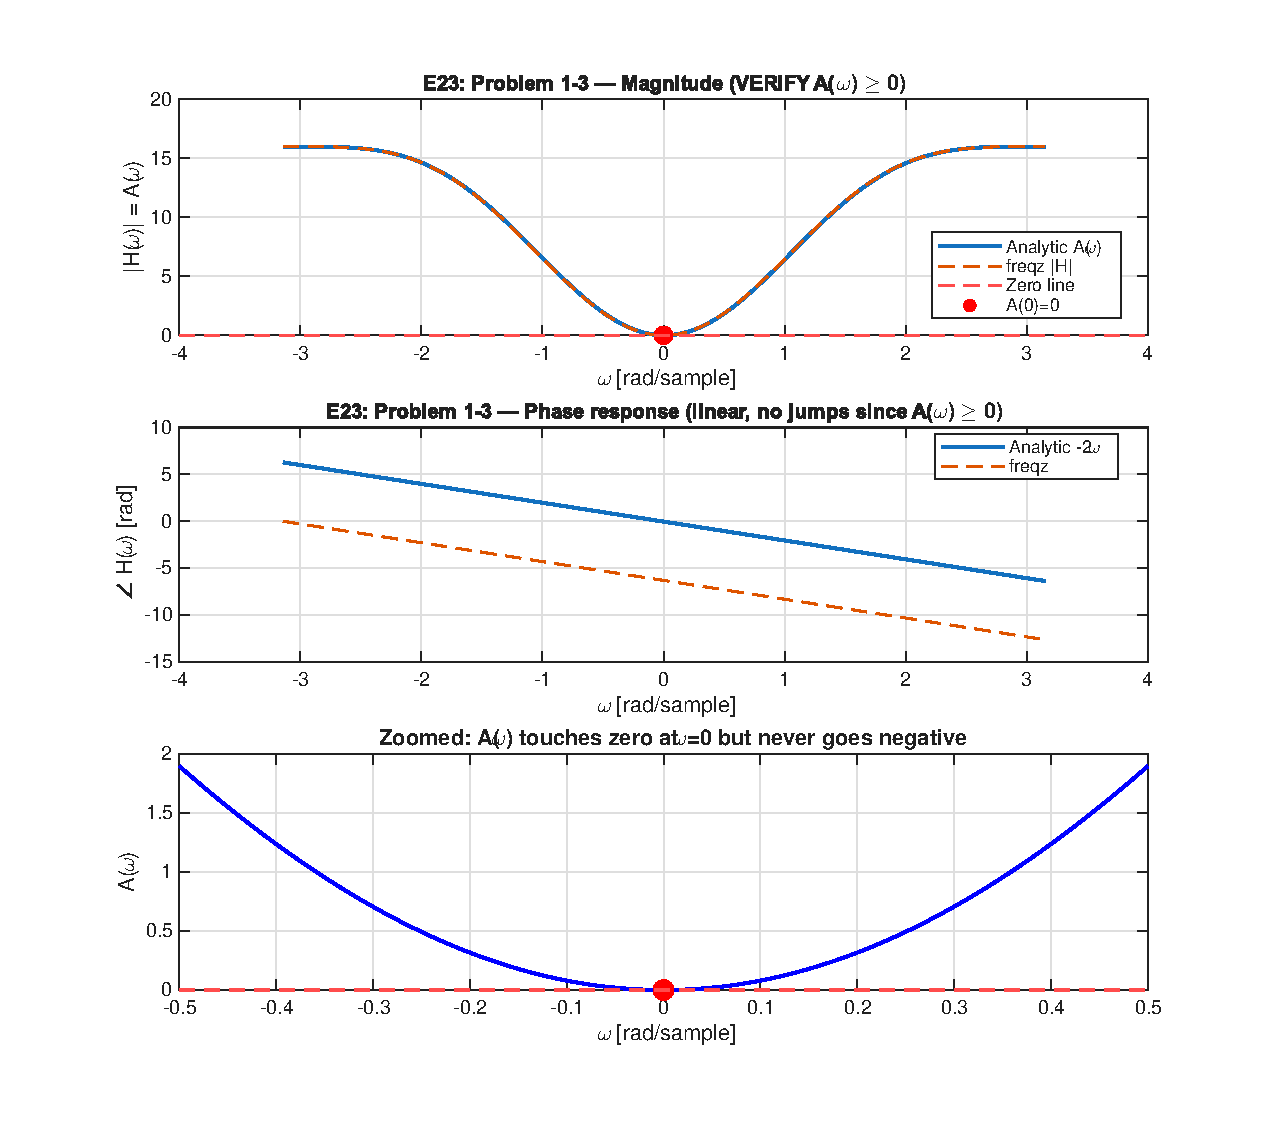
\includegraphics[width=\maxwidth{80.28098344204717em}]{figure_1.eps}
\end{center}
\begin{matlabcode}


\end{matlabcode}


\matlabheading{1-4) Second FIR filter H2(z) in cascade}

\begin{matlabcode}

% Overall H(z) has numerator B = h.
% First filter: H1(z) = 1 - z^{-1}  ⇒ polynomial [1 -1]
H1 = [1 -1];

% Deconvolution: B = conv(H1, H2_num)
[H2_num, rem_poly] = deconv(B, H1);

fprintf('\n1-4) H2(z) numerator coefficients:\n');
\end{matlabcode}
\begin{matlaboutput}
1-4) H2(z) numerator coefficients:
\end{matlaboutput}
\begin{matlabcode}
disp(H2_num);
\end{matlabcode}
\begin{matlaboutput}
    -1    -5     5     1
\end{matlaboutput}
\begin{matlabcode}
fprintf('Deconvolution remainder (should be near zero):\n');
\end{matlabcode}
\begin{matlaboutput}
Deconvolution remainder (should be near zero):
\end{matlaboutput}
\begin{matlabcode}
disp(rem_poly);
\end{matlabcode}
\begin{matlaboutput}
     0     0     0     0     0
\end{matlaboutput}
\begin{matlabcode}

% Pole-zero plot of H2(z) (FIR, so only zeros)
figure;
zplane(H2_num, 1);
title('E23: Problem 1-4 — Pole-zero plot of H_2(z)');
exportgraphics(gcf, fullfile(imgDir, ...
    'DSP_Exam_E23_1_H2_PZ.png'), 'Resolution', 300);
\end{matlabcode}
\begin{center}
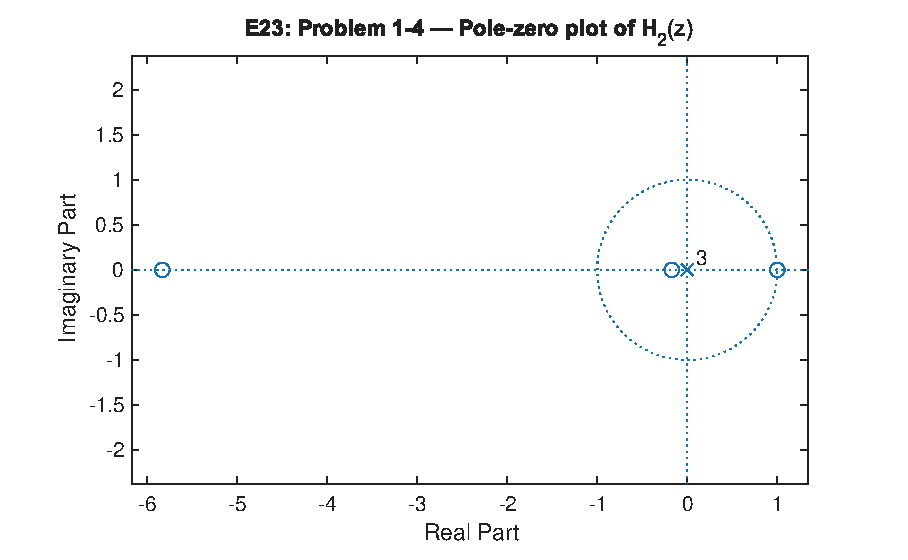
\includegraphics[width=\maxwidth{56.196688409433015em}]{figure_2.eps}
\end{center}
\begin{matlabcode}



\end{matlabcode}


\matlabheading{Problem 2 — IIR High-pass Chebyshev Type I via BLT}

\begin{matlabcode}

Fs_IIR = 4000;                 % sampling frequency [Hz]
Ts_IIR = 1/Fs_IIR;
Ap_dB = 3;                     % passband ripple [dB]
As_dB = 30;                    % stopband attenuation [dB]

Fp_HP = 700;                   % passband edge [Hz]
Fs_stop_HP = 400;              % stopband edge [Hz]


\end{matlabcode}


\matlabheading{2-1) Chebyshev prototype: epsilon, prewarping, order and prototype TF}

\begin{matlabcode}

eps2 = 10^(Ap_dB/10) - 1;
eps_val = sqrt(eps2);

fprintf('\n2-1) Chebyshev Type I ε = %.4f\n', eps_val);
\end{matlabcode}
\begin{matlaboutput}
2-1) Chebyshev Type I ε = 0.9976
\end{matlaboutput}
\begin{matlabcode}

prewarp = @(F) 2*Fs_IIR*tan(pi*F/Fs_IIR);
Omegap_HP = prewarp(Fp_HP);
Omegas_HP = prewarp(Fs_stop_HP);

fprintf('Prewarped analog edges:\n');
\end{matlabcode}
\begin{matlaboutput}
Prewarped analog edges:
\end{matlaboutput}
\begin{matlabcode}
fprintf('  Omegap = %.2f rad/s (from Fp = %g Hz)\n', Omegap_HP, Fp_HP);
\end{matlabcode}
\begin{matlaboutput}
  Omegap = 4902.41 rad/s (from Fp = 700 Hz)
\end{matlaboutput}
\begin{matlabcode}
fprintf('  Omegas = %.2f rad/s (from Fs = %g Hz)\n', Omegas_HP, Fs_stop_HP);
\end{matlabcode}
\begin{matlaboutput}
  Omegas = 2599.36 rad/s (from Fs = 400 Hz)
\end{matlaboutput}
\begin{matlabcode}

Gp = 10^(-Ap_dB/20);
Gs = 10^(-As_dB/20);
k1 = sqrt(1/Gs^2 - 1);
k2 = sqrt(1/Gp^2 - 1);

n_cheb = acosh(k1/k2) / acosh(Omegas_HP/Omegap_HP);
n_min  = ceil(n_cheb);

fprintf('Chebyshev order estimate = %.3f -> n_min = %d\n', n_cheb, n_min);
\end{matlabcode}
\begin{matlaboutput}
Chebyshev order estimate = 0.000 -> n_min = 0
\end{matlaboutput}
\begin{matlabcode}

% From appendix: order-4 Chebyshev Type I LP prototype (3 dB)
B_proto = 0.1253;
A_proto = [1 0.5816 1.1691 0.4048 0.1770];

sys_proto = tf(B_proto, A_proto);
disp('2-1) Chebyshev Type I LP prototype (n=4):');
\end{matlabcode}
\begin{matlaboutput}
2-1) Chebyshev Type I LP prototype (n=4):
\end{matlaboutput}
\begin{matlabcode}
sys_proto
\end{matlabcode}
\begin{matlaboutput}
sys_proto =
 
                      0.1253
  -----------------------------------------------
  s^4 + 0.5816 s^3 + 1.169 s^2 + 0.4048 s + 0.177
 
Continuous-time transfer function.
Model Properties
\end{matlaboutput}
\begin{matlabcode}


\end{matlabcode}


\matlabheading{2-2) Analog high-pass H\_HP(s) via LP -\textgreater{} HP transform}

\begin{matlabcode}

[B_HP, A_HP] = lp2hp(B_proto, A_proto, Omegap_HP);
sys_HP = tf(B_HP, A_HP);
disp('2-2) Analog HP Chebyshev filter H_HP(s):');
\end{matlabcode}
\begin{matlaboutput}
2-2) Analog HP Chebyshev filter H_HP(s):
\end{matlaboutput}
\begin{matlabcode}
sys_HP
\end{matlabcode}
\begin{matlaboutput}
sys_HP =
 
  0.7079 s^4 + 4.59e-12 s^3 + 3.789e-08 s^2 + 0.0001292 s + 0.4291
  ----------------------------------------------------------------
     s^4 + 1.121e04 s^3 + 1.587e08 s^2 + 3.871e11 s + 3.263e15
 
Continuous-time transfer function.
Model Properties
\end{matlaboutput}
\begin{matlabcode}

Omega = linspace(0, 2.5*Omegap_HP, 4000);  % rad/s
H_HP = freqs(B_HP, A_HP, Omega);

F_analog = Omega/(2*pi);                    % Hz
Mag_HP_dB = 20*log10(abs(H_HP));

figure;
plot(F_analog, Mag_HP_dB, 'LineWidth', 1.5); grid on;
xlabel('Analog frequency F [Hz]');
ylabel('|H_{HP}(j\Omega)| [dB]');
title('E23: Problem 2-2 — Analog HP Chebyshev magnitude');
xline(Fs_stop_HP, '--r', 'F_s = 400 Hz');
xline(Fp_HP,      '--g', 'F_p = 700 Hz');

exportgraphics(gcf, fullfile(imgDir, ...
    'DSP_Exam_E23_2_Analog_HP_Mag_dB.png'), 'Resolution', 300);
\end{matlabcode}
\begin{center}
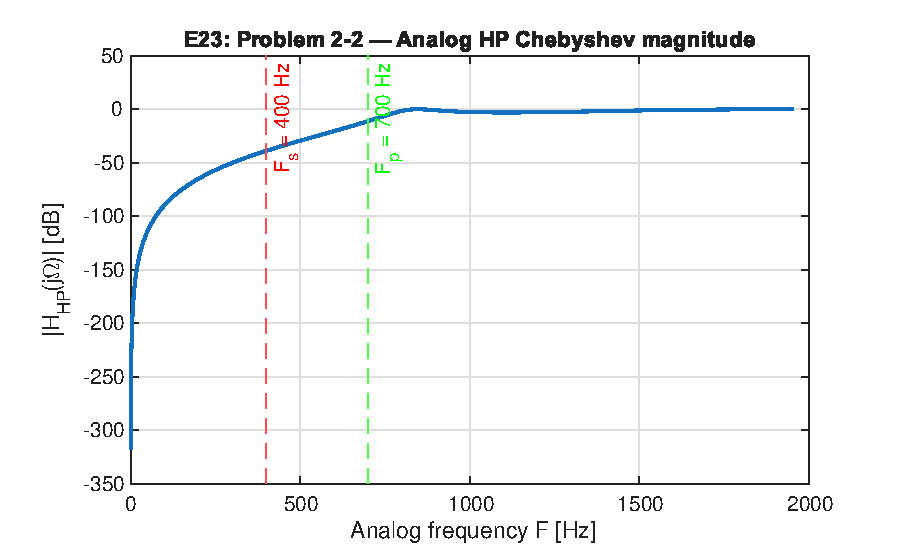
\includegraphics[width=\maxwidth{56.196688409433015em}]{figure_3.eps}
\end{center}
\begin{matlabcode}


\end{matlabcode}


\matlabheading{2-3) Digital high-pass H\_HP(z) via Bilinear Transform}

\begin{matlabcode}

[Bz_HP, Az_HP] = bilinear(B_HP, A_HP, Fs_IIR);
\end{matlabcode}
\begin{matlaboutput}
Warning: Matrix is close to singular or badly scaled. Results may be inaccurate. RCOND =  3.866585e-23.
Warning: Matrix is close to singular or badly scaled. Results may be inaccurate. RCOND =  3.866585e-23.
Warning: Matrix is close to singular or badly scaled. Results may be inaccurate. RCOND =  3.865667e-23.
Warning: Matrix is close to singular or badly scaled. Results may be inaccurate. RCOND =  3.865667e-23.
\end{matlaboutput}
\begin{matlabcode}

sys_HP_z = tf(Bz_HP, Az_HP, Ts_IIR, 'Variable', 'z^-1');
disp('2-3) Digital HP Chebyshev H_HP(z):');
\end{matlabcode}
\begin{matlaboutput}
2-3) Digital HP Chebyshev H_HP(z):
\end{matlaboutput}
\begin{matlabcode}
sys_HP_z
\end{matlabcode}
\begin{matlaboutput}
sys_HP_z =
 
  0.11 - 0.4401 z^-1 + 0.6601 z^-2 - 0.4401 z^-3 + 0.11 z^-4
  ----------------------------------------------------------
  1 - 0.3269 z^-1 + 0.9044 z^-2 + 0.07421 z^-3 + 0.3294 z^-4
 
Sample time: 0.00025 seconds
Discrete-time transfer function.
Model Properties
\end{matlaboutput}
\begin{matlabcode}


\end{matlabcode}


\matlabheading{2-4) Digital magnitude and attenuation at spec edges}

\begin{matlabcode}

F_resp = linspace(0, Fs_IIR/2, 4000);    % 0..Nyquist
[Hdig_HP, Fgrid_HP] = freqz(Bz_HP, Az_HP, F_resp, Fs_IIR);
Magdig_HP_dB = 20*log10(abs(Hdig_HP));

figure;
plot(Fgrid_HP, Magdig_HP_dB, 'LineWidth', 1.5); grid on;
xlabel('f [Hz]');
ylabel('|H_{HP}(e^{j\omega})| [dB]');
title('E23: Problem 2-4 — Digital HP Chebyshev magnitude');
xline(Fs_stop_HP, '--r', 'F_s = 400 Hz');
xline(Fp_HP,      '--g', 'F_p = 700 Hz');

exportgraphics(gcf, fullfile(imgDir, ...
    'DSP_Exam_E23_2_Digital_HP_Mag_dB.png'), 'Resolution', 300);
\end{matlabcode}
\begin{center}
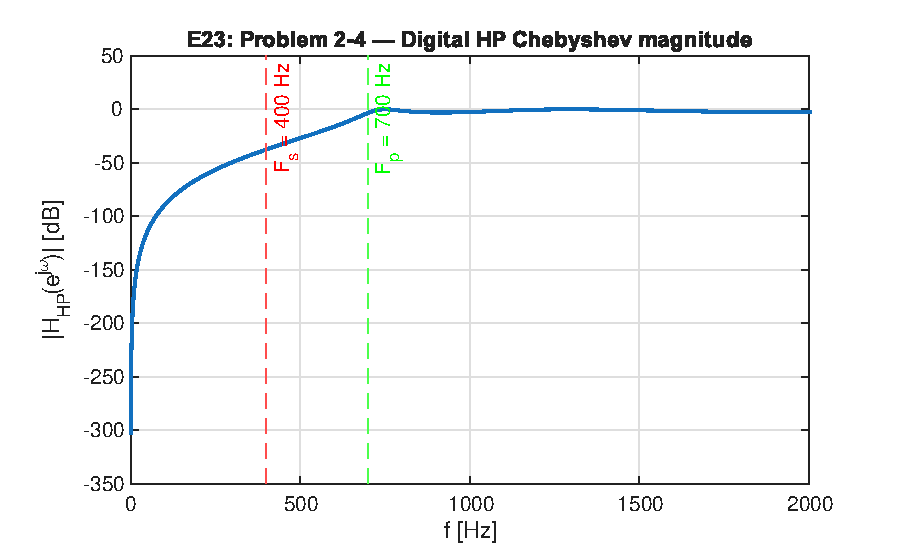
\includegraphics[width=\maxwidth{56.196688409433015em}]{figure_4.eps}
\end{center}
\begin{matlabcode}

F_edges_HP = [Fs_stop_HP, Fp_HP];
[H_edges_HP, ~] = freqz(Bz_HP, Az_HP, F_edges_HP, Fs_IIR);
Att_edges_dB_HP = 20*log10(abs(H_edges_HP));

fprintf('\nDigital HP attenuation at key edges:\n');
\end{matlabcode}
\begin{matlaboutput}
Digital HP attenuation at key edges:
\end{matlaboutput}
\begin{matlabcode}
fprintf('  At %g Hz (stopband): %.2f dB\n', Fs_stop_HP, Att_edges_dB_HP(1));
\end{matlabcode}
\begin{matlaboutput}
  At 400 Hz (stopband): -37.34 dB
\end{matlaboutput}
\begin{matlabcode}
fprintf('  At %g Hz (passband): %.2f dB\n', Fp_HP,      Att_edges_dB_HP(2));
\end{matlabcode}
\begin{matlaboutput}
  At 700 Hz (passband): -3.00 dB
\end{matlaboutput}
\begin{matlabcode}


\end{matlabcode}


\matlabheading{Problem 3 — Sampling \& IIR ROC / Inverse (illustrative plots)}

\begin{matlabcode}

% This part is mainly conceptual in the exam; we add a generic ROC example.


%% 3-3) Example pole-zero plot & ROC idea
B_ex = [1 0];                % example zero at z = 0
A_ex = [1 -0.8 0.64];        % example poles inside unit circle

figure;
zplane(B_ex, A_ex);
title('E23: Problem 3-3 — Example pole-zero plot & ROC');
exportgraphics(gcf, fullfile(imgDir, ...
    'DSP_Exam_E23_3_PZ_ROC.png'), 'Resolution', 300);
\end{matlabcode}
\begin{center}
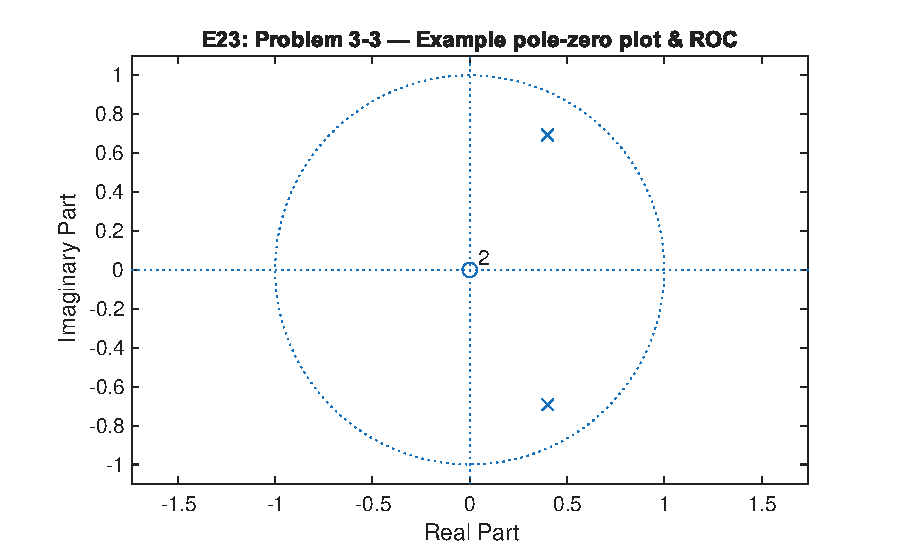
\includegraphics[width=\maxwidth{56.196688409433015em}]{figure_5.eps}
\end{center}
\begin{matlabcode}


\end{matlabcode}


\matlabheading{Problem 4 — FIR High-pass via Fourier Series + Spectrum}

\begin{matlabcode}

Fs_FIR = 2000;               % sampling frequency used in Problem 4
Ts_FIR = 1/Fs_FIR;
Fc_HP_FIR = 240;             % (nominal cutoff, for reference)


\end{matlabcode}


\matlabheading{4-1) High-pass FIR coefficients and magnitude}

\begin{matlabcode}

b_hp = [ ...
   0.038394   0.052112   0.037420  -0.0099737  -0.081754 ...
  -0.15884   -0.21790    0.76000   -0.21790    -0.15884  ...
  -0.081754  -0.0099737  0.037420   0.052112    0.038394 ];
a_hp = 1;

n_hp = 0:length(b_hp)-1;

figure;
stem(n_hp, b_hp, 'filled'); grid on;
xlabel('n');
ylabel('h_{HP}[n]');
title('E23: Problem 4-1 — High-pass FIR impulse response');
exportgraphics(gcf, fullfile(imgDir, ...
    'DSP_Exam_E23_4_HP_Impulse.png'), 'Resolution', 300);
\end{matlabcode}
\begin{center}
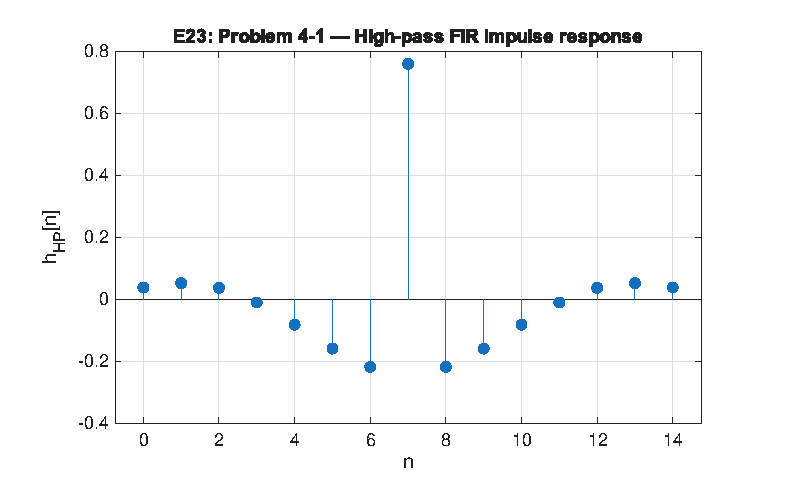
\includegraphics[width=\maxwidth{56.196688409433015em}]{figure_6.eps}
\end{center}
\begin{matlabcode}

[H_hp, F_hp] = freqz(b_hp, a_hp, 4096, Fs_FIR);
Mag_hp_dB = 20*log10(abs(H_hp));

figure;
plot(F_hp, Mag_hp_dB, 'LineWidth', 1.5); grid on;
xlabel('f [Hz]');
ylabel('|H_{HP}(e^{j\omega})| [dB]');
title('E23: Problem 4-1 — High-pass FIR magnitude (dB)');
xline(100, '--r', '100 Hz');
xline(350, '--g', '350 Hz');
exportgraphics(gcf, fullfile(imgDir, ...
    'DSP_Exam_E23_4_HP_FIR_Mag_dB.png'), 'Resolution', 300);
\end{matlabcode}
\begin{center}
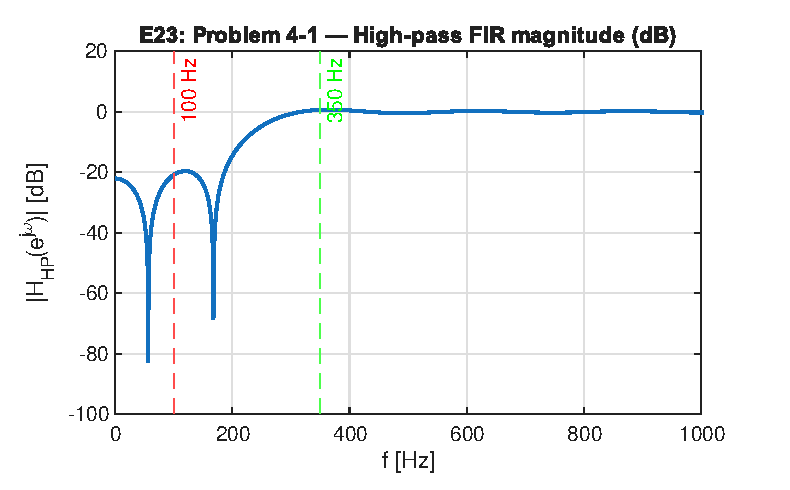
\includegraphics[width=\maxwidth{56.196688409433015em}]{figure_7.eps}
\end{center}
\begin{matlabcode}


\end{matlabcode}


\matlabheading{4-2) Spectrum of sampled 2-tone signal x[n]}

\begin{matlabcode}

N_sig = 4096;                        % number of samples (can adjust)
n_sig = 0:N_sig-1;
t_sig = n_sig * Ts_FIR;

F1 = 100;   A1 = 6;
F2 = 350;   A2 = 2;

x = A1*sin(2*pi*F1*t_sig) + A2*cos(2*pi*F2*t_sig);

X = fft(x);
Xs = fftshift(X) / N_sig;

f_axis = (-N_sig/2:N_sig/2-1)*(Fs_FIR/N_sig);

figure;
plot(f_axis, abs(Xs), 'LineWidth', 1); grid on;
xlabel('F [Hz]');
ylabel('|X(F)| (scaled)');
title('E23: Problem 4-2 — Spectrum of x[n]');
xlim([-500 500]);
exportgraphics(gcf, fullfile(imgDir, ...
    'DSP_Exam_E23_4_InputSpectrum.png'), 'Resolution', 300);
\end{matlabcode}
\begin{center}
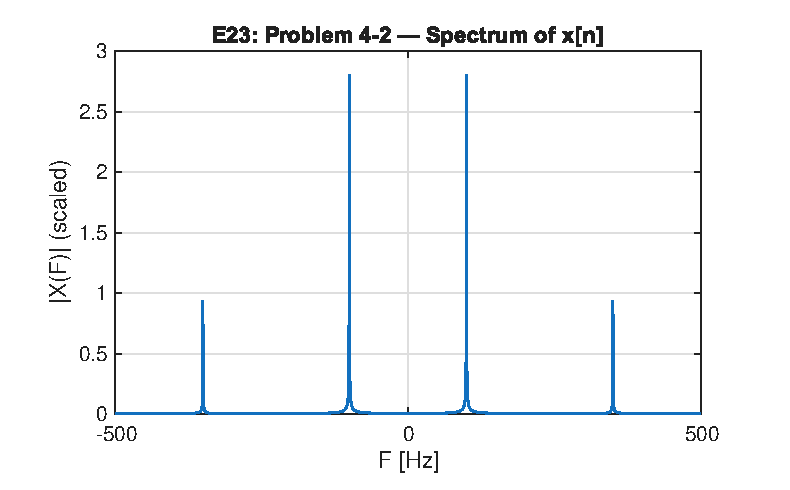
\includegraphics[width=\maxwidth{56.196688409433015em}]{figure_8.eps}
\end{center}
\begin{matlabcode}

targetFreqs = [100 350];
for F0 = targetFreqs
    [~, idx_pos] = min(abs(f_axis - F0));
    [~, idx_neg] = min(abs(f_axis + F0));
    fprintf('\nApprox |X| at ±%d Hz: %.3f (pos), %.3f (neg)\n', ...
        F0, abs(Xs(idx_pos)), abs(Xs(idx_neg)));
end
\end{matlabcode}
\begin{matlaboutput}
Approx |X| at ±100 Hz: 2.807 (pos), 2.807 (neg)

Approx |X| at ±350 Hz: 0.937 (pos), 0.937 (neg)
\end{matlaboutput}
\begin{matlabcode}


\end{matlabcode}


\matlabheading{4-3) Output spectrum after HP filtering}

\begin{matlabcode}

y = filter(b_hp, a_hp, x);

Y = fft(y);
Ys = fftshift(Y) / N_sig;

figure;
plot(f_axis, abs(Ys), 'LineWidth', 1); grid on;
xlabel('F [Hz]');
ylabel('|Y(F)| (scaled)');
title('E23: Problem 4-3 — Spectrum after HP filtering');
xlim([-500 500]);
exportgraphics(gcf, fullfile(imgDir, ...
    'DSP_Exam_E23_4_OutputSpectrum.png'), 'Resolution', 300);
\end{matlabcode}
\begin{center}
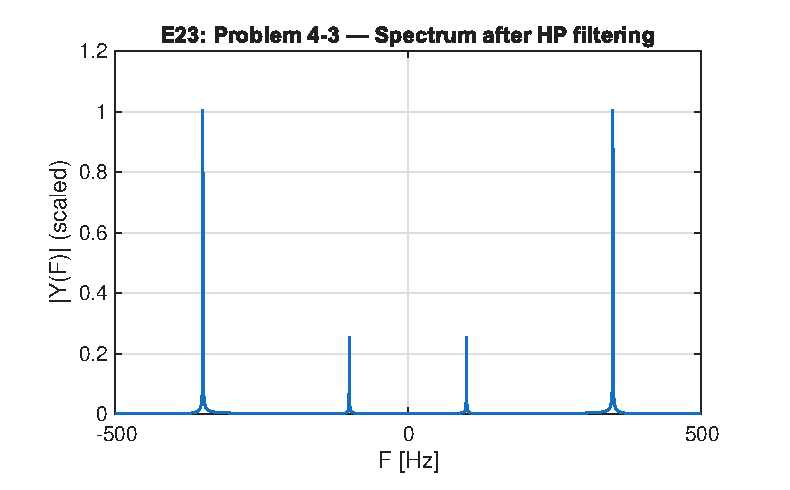
\includegraphics[width=\maxwidth{56.196688409433015em}]{figure_9.eps}
\end{center}
\begin{matlabcode}

for F0 = targetFreqs
    [~, idx_pos] = min(abs(f_axis - F0));
    [~, idx_neg] = min(abs(f_axis + F0));
    fprintf('Approx |Y| at ±%d Hz: %.4f (pos), %.4f (neg)\n', ...
        F0, abs(Ys(idx_pos)), abs(Ys(idx_neg)));
end
\end{matlabcode}
\begin{matlaboutput}
Approx |Y| at ±100 Hz: 0.2552 (pos), 0.2552 (neg)
Approx |Y| at ±350 Hz: 1.0093 (pos), 1.0093 (neg)
\end{matlaboutput}
\begin{matlabcode}

fprintf('\n========================================\n');
\end{matlabcode}
\begin{matlaboutput}
========================================
\end{matlaboutput}
\begin{matlabcode}
fprintf('E23 exam MATLAB companion finished.\n');
\end{matlabcode}
\begin{matlaboutput}
E23 exam MATLAB companion finished.
\end{matlaboutput}
\begin{matlabcode}
fprintf('All figures exported to:\n%s\n', imgDir);
\end{matlabcode}
\begin{matlaboutput}
All figures exported to:
C:\Users\Mads2\DTU\Obsidian\Courses\DSP\Images
\end{matlaboutput}
\begin{matlabcode}
fprintf('========================================\n');
\end{matlabcode}
\begin{matlaboutput}
========================================
\end{matlaboutput}

\end{document}
